\chapter{Detalles de Implementación y Experimentos}\label{chapter:implementation}

El estudio se realiz\'o en un sistema operativo GNU/Linux 22.04 LTS con una CPU Intel Core i3-5020U 2.20Ghz y 12GB de RAM a 1600MHz de velocidad. Se utiliz\'o Docker 19.03.8 para las im\'agenes de Fabric v2.4.\\

Para configurar la red se utiliz\'o Minifabric en su versi\'on m\'as reciente. Las pruebas de rendimiento se realizaron con Caliper v0.5.0 empleando el \emph{chaincode} \emph{samplecc} suministrado por Minifabric.\\

El nodo ordenador emple\'o el mecanismo de consenso \emph{raft} en cada una de las configuraciones y los nodos pares, \emph{GoLevelDB} como base de datos de estado. Se destaca el uso del voto por mayor\'ia en la pol\'itica de aprobaci\'on, donde todos los nodos pares fueron igualmente configurados para participar en ella. Se tuvo en cuenta el estudio en una sola organizaci\'on, pero de acuerdo a la pol\'itica de aprobaci\'on implantada, su comportamiento simula para $n$ nodos pares, una red con $n$ organizaciones de un nodo par cada una, donde se evita el sesgo que propicia la conectividad en las organizaciones.

\newpage
\section{Escenario de bajo volumen de transacciones}

En las tablas \ref{tab:10TPS-10BS}, \ref{tab:10TPS-50BS} y \ref{tab:10TPS-100BS} se registran los datos obtenidos para el escenario de 10 TPS.\\

\subsection{An\'alisis de latencia}
De acuerdo a los datos suministrados se puede visualizar el comportamiento de las medidas de latencia para las configuraciones con diferente tama\~no en los bloques del canal.\\

\begin{figure}[htbp]
\subfigure[Tama\~no de bloque igual 10.]{
\begin{minipage}[t]{0.30\linewidth}
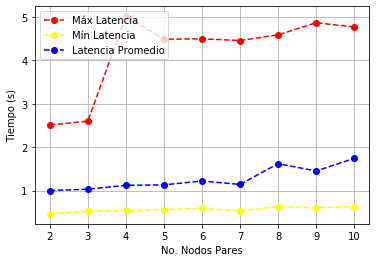
\includegraphics[scale=0.35]{Graphics/AnalisisLatenciaPares10TPSBS10.png}
\end{minipage}
}
\subfigure[Tama\~no de bloque igual 50.]{
\begin{minipage}[t]{0.30\linewidth}
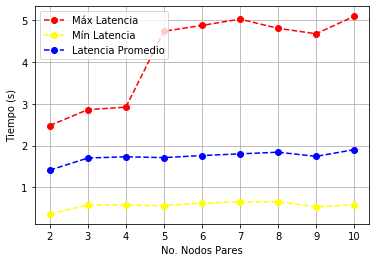
\includegraphics[scale=0.35]{Graphics/AnalisisLatenciaPares10TPSBS50.png}
\end{minipage}
}
\subfigure[Tama\~no de bloque igual 100.]{
\begin{minipage}[t]{0.30\linewidth}
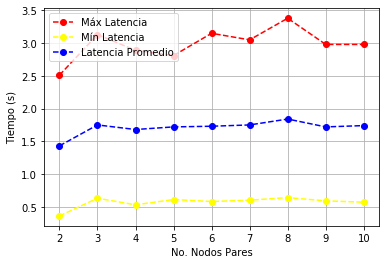
\includegraphics[scale=0.35]{Graphics/AnalisisLatenciaPares10TPSBS100.png}
\end{minipage}
}
\caption{Comportamiento de la latencia en distintas configuraciones de redes con un n\'umero variable de nodos pares y tama\~nos de bloques en escenarios de 10 TPS.}
\end{figure}

De acuerdo a la latencia m\'inima, para los tres casos mantienen un comportamiento similar, marcado por una leve tendencia al crecimiento con el aumento del n\'umero de nodos pares en la red. En el caso de la red configurada con un tama\~no de bloque igual a 10, los valores de latencia promedio son m\'as pr\'oximos a los valores de latencia m\'inima con respecto a las dem\'as configuraciones. Esto sucede porque al llegar las transacciones al servicio de ordenaci\'on, como el tama\~no del bloque es menor que el resto, y a su vez tiene una capacidad no superior al n\'umero de transacciones suministradas por los clientes, el tiempo de espera, en promedio, de las transacciones v\'alidas para cerrar el bloque es menor. Esta afirmaci\'on contrasta con la latencia m\'axima que, a menor tama\~no de bloque, mayores valores alcanza producto a que ocurre un proceso de llenado m\'as r\'apido originando una validaci\'on m\'as frecuente en los nodos pares, que a su vez participan en el proceso de simulaci\'on de las transacciones elevando la probabilidad de saturaci\'on en su proceso de ejecuci\'on.\\

En la figura \ref{ComparacionLatencia10TPS} se percibe que para un tama\~no de bloque igual a 10, el valor de latencia promedio es m\'inimo para todos las configuraciones de nodos pares. Luego, el tama\~no de bloque 10 es un par\'ametro que optimiza la latencia promedio en la red, en comparaci\'on a los dem\'as, por tanto, es un posible candidato a \'optimo.\\

\begin{figure}[h]
\centering
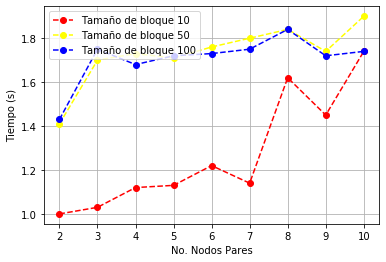
\includegraphics[scale=0.5]{Graphics/ComparacionLatencia10TPS.png}
\caption{Latencia promedio en redes con distinto tama\~no de bloque para escenarios de 10 TPS.}
\label{ComparacionLatencia10TPS}
\end{figure}


\subsection{An\'alisis de rendimiento}

\begin{figure}[h]
\subfigure[Tama\~no de bloque igual 10.]{
\begin{minipage}[t]{0.30\linewidth}
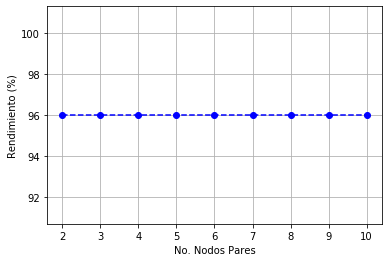
\includegraphics[scale=0.35]{Graphics/RendimientoPares10TPSBS10.png}
\end{minipage}
}
\subfigure[Tama\~no de bloque igual 50.]{
\begin{minipage}[t]{0.30\linewidth}
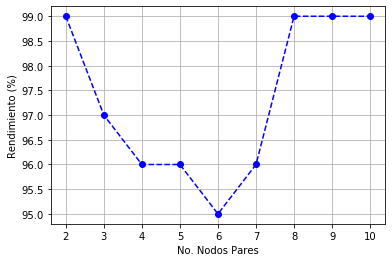
\includegraphics[scale=0.35]{Graphics/RendimientoPares10TPSBS50.png}
\end{minipage}
}
\subfigure[Tama\~no de bloque igual 100.]{
\begin{minipage}[t]{0.30\linewidth}
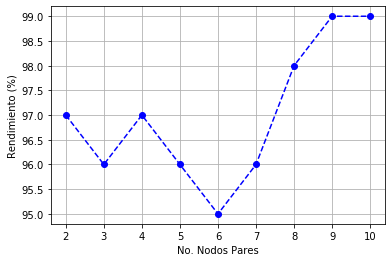
\includegraphics[scale=0.35]{Graphics/RendimientoPares10TPSBS100.png}
\end{minipage}
}
\caption{Comportamiento del rendimiento en distintas configuraciones de redes con un n\'umero variable de nodos pares y tama\~nos de bloques en escenarios de 10 TPS.}
\end{figure}


Para los tama\~nos de bloques planteados, los valores de rendimiento de la red oscilan entre el 95$\%$ y 99$\%$. La red configurada con tama\~no de bloque 10 mantiene un rendimiento constante de 96$\%$ para las configuraciones de nodos pares estudiadas.\\

 En el caso de la red con bloques de tama\~no 50 se alcanza un mejor rendimiento en la mayor\'ia de las configuraciones de nodos pares, como se puede ver en la figura \ref{RendimientoPares10TPS}.\\

\begin{figure}[h]
\centering
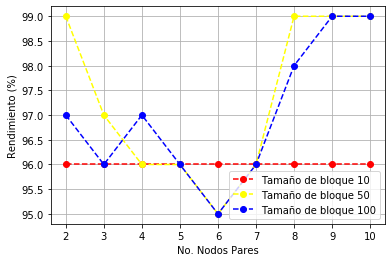
\includegraphics[scale=0.5]{Graphics/RendimientoPares10TPS.png}
\caption{Rendimiento de redes con distinto tama\~no de bloque para escenarios de 10 TPS.}
\label{RendimientoPares10TPS}
\end{figure}

\newpage

Para determinar una configuraci\'on \'optima, en relaci\'on a los valores de los par\'ametros estudiados, se tuvo en cuenta el rendimiento en la red y la latencia promedio. Para establecer una comparaci\'on se llevaron las m\'etricas a una escala global, normalizando sus valores. Estos valores son estimaciones promedio para configuraciones con una cantidad de nodos pares entre dos y diez por organizaci\'on, donde el tama\~no de los bloques representa el factor de decisi\'on. En la figura \ref{Resultado10TPS} podemos ver que el mejor rendimiento se alcanza para canales con tama\~no de bloque igual a 50, pero a su vez la latencia promedio es mayor que la estimada para las configuraciones de canales de tama\~no 10. Por tanto, los valores 10 y 50 representan \'optimos locales, que en dependencia del escenario de uso, minimizan la latencia promedio y maximizan el rendimiento de la red respectivamente.\\

\begin{figure}[h]
\centering
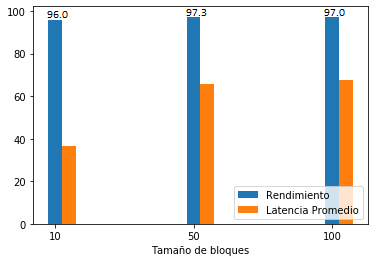
\includegraphics[scale=0.7]{Graphics/Resultado10TPS.png}
\caption{Evaluaci\'on de resultados para escenarios de 10 TPS.}
\label{Resultado10TPS}
\end{figure}

\newpage

\section{Escenario de alto volumen de transacciones}

En las tablas \ref{tab:100TPS-10BS}, \ref{tab:100TPS-50BS} y \ref{tab:100TPS-100BS} se registran los datos obtenidos para el escenario de 100 TPS.\\

\subsection{An\'alisis de latencia}

Las siguientes gr\'aficas muestran el comportamiento de las medidas de latencia para las configuraciones con diferente tama\~no en los bloques del canal.\\

\begin{figure}[htbp]
\subfigure[Tama\~no de bloque igual 10.]{
\begin{minipage}[t]{0.30\linewidth}
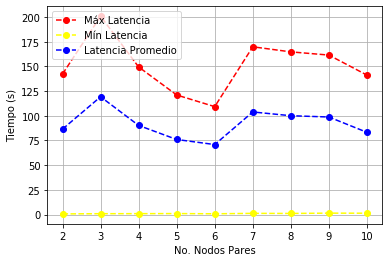
\includegraphics[scale=0.35]{Graphics/AnalisisLatenciaPares100TPSBS10.png}
\end{minipage}
}
\subfigure[Tama\~no de bloque igual 50.]{
\begin{minipage}[t]{0.30\linewidth}
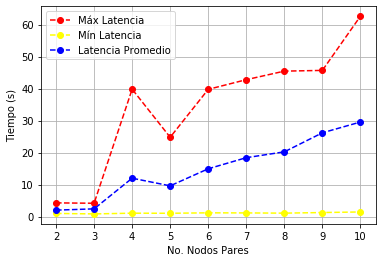
\includegraphics[scale=0.35]{Graphics/AnalisisLatenciaPares100TPSBS50.png}
\end{minipage}
}
\subfigure[Tama\~no de bloque igual 100.]{
\begin{minipage}[t]{0.30\linewidth}
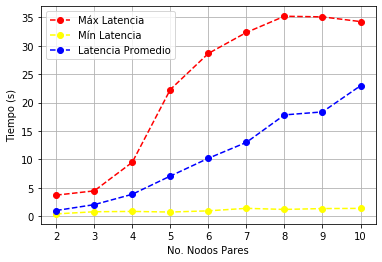
\includegraphics[scale=0.35]{Graphics/AnalisisLatenciaPares100TPSBS100.png}
\end{minipage}
}
\caption{Comportamiento de la latencia en distintas configuraciones de redes con un n\'umero variable de nodos pares y tama\~nos de bloques en escenarios de 100 TPS.}
\end{figure}


En la primera gr\'afica podemos observar que los valores de latencia promedio oscilan entre los 70 y 120 segundos aproximadamente. Estos valores son, en extremo, elevados en comparaci\'on con las restantes configuraciones. Para el caso de los bloques de tama\~no 100 el mayor valor alcanzado de latencia promedio, no supera los 25 segundos, quedando todos sus valores por debajo de los alcanzados por la configuraci\'on de bloques de tama\~no 10. Lo mismo sucede en las redes con bloques de tama\~no 50 que no superan los 30 segundos.\\

Para determinar el tama\~no de bloque que ofrece mejor desempe\~no en redes con un n\'umero de nodos pares que var\'ia de dos a diez por organizaci\'on,  con respecto a la latencia de las transacciones, se calcul\'o la media de las latencias promedios de las configuraciones de nodos pares, por tama\~nos de bloques, y nos quedamos con la configuraci\'on de bloque que corresponda a la menor de ellas.\\

Los bloques de tama\~no 10, 50 y 100 promedian una latencia media para las configuraciones de nodos pares de 92.1, 15.0 y 10.7 segundos respectivamente. Por tanto, las redes configuradas con bloques de tama\~no 100 son \'optimas respecto al conjunto estudiado, propiciando la menor latencia promedio. Para establecer una comparativa visual nos podemos remitir a la figura \ref{ComparacionLatencia100TPS}.\\

\begin{figure}[h]
\centering
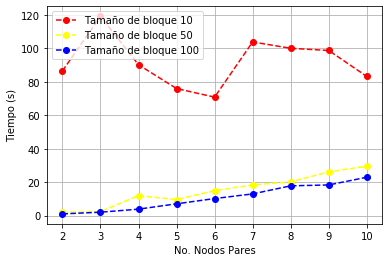
\includegraphics[scale=0.5]{Graphics/ComparacionLatencia100TPS.png}
\caption{Latencia promedio en redes con distinto tama\~no de bloque para escenarios de 100 TPS.}
\label{ComparacionLatencia100TPS}
\end{figure}

\subsection{An\'alisis de rendimiento}

\begin{figure}[h]
\subfigure[Tama\~no de bloque igual 10.]{
\begin{minipage}[t]{0.30\linewidth}
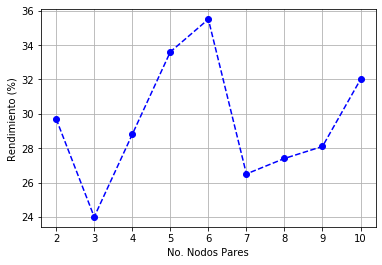
\includegraphics[scale=0.35]{Graphics/RendimientoPares100TPSBS10.png}
\end{minipage}
}
\subfigure[Tama\~no de bloque igual 50.]{
\begin{minipage}[t]{0.30\linewidth}
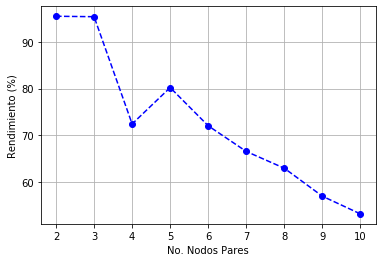
\includegraphics[scale=0.35]{Graphics/RendimientoPares100TPSBS50.png}
\end{minipage}
}
\subfigure[Tama\~no de bloque igual 100.]{
\begin{minipage}[t]{0.30\linewidth}
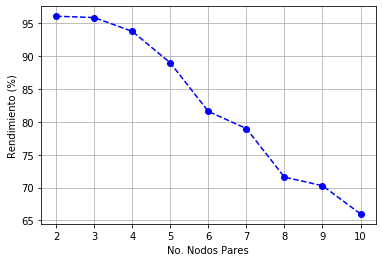
\includegraphics[scale=0.35]{Graphics/RendimientoPares100TPSBS100.png}
\end{minipage}
}
\caption{Comportamiento del rendimiento en distintas configuraciones de redes con un n\'umero variable de nodos pares y tama\~nos de bloques en escenarios de 100 TPS.}
\end{figure}

De acuerdo a la gr\'afica que representa el rendimiento para las redes con bloques de tama\~no 10, se destaca el bajo rendimiento que logran en escenarios de altos vol\'umenes de transacciones. Entre las causas fundamentales que lo ocasionan est\'a el r\'apido llenado de los bloques por el servicio de ordenaci\'on, que luego son enviados, con mayor frecuencia, a los nodos pares para el proceso de validaci\'on y a su vez se conjuga con el alto volumen de transacciones que deben simular en cada intervalo de tiempo, provocando una mayor demora en el procesamiento y elevando la probabilidad de fallos. Los bloques de tama\~no 50 y 100 manifiestan un mejor rendimiento debido a que compensan la frecuencia de validaci\'on por los nodos pares, con un aumento del tiempo de conformaci\'on de bloques.\\

Si ilustramos las curvas de rendimiento en una sola gr\'afica, como en la figura \ref{RendimientoPares100TPS}, apreciamos que las redes con bloques de tama\~no 100 superan para todas las configuraciones de nodos pares, a las redes con bloques de tama\~no inferior. Se aprecia adem\'as, que para escenarios de altos vol\'umenes de transacciones por segundo, el aumento del n\'umero de nodos pares en las organizaciones reducen el rendimiento de forma considerable.

\begin{figure}[h]
\centering
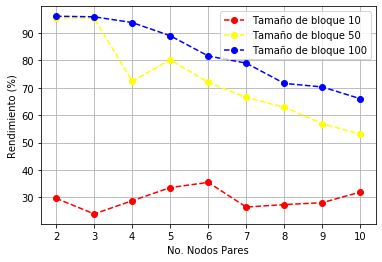
\includegraphics[scale=0.5]{Graphics/RendimientoPares100TPS.png}
\caption{Rendimiento de redes con distinto tama\~no de bloque para escenarios de 100 TPS.}
\label{RendimientoPares100TPS}
\end{figure}

\newpage

En este escenario, la configuraci\'on para bloques de tama\~no 100, propicia la menor latencia promedio en la red y el mejor desempe\~no en el rendimiento, del conjunto evaluado. En la figura \ref{Resultado100TPS} se puede ver el marcado contraste dado por la diferencia en el tama\~no de los bloques. Se tiene una diferencia m\'axima de latencia superior a los 80 segundos, igual comportamiento tenemos en el rendimiento, donde los bloque de tama\~no 10 ofrecen las m\'etricas m\'as desfavorables. A su vez, esta coincide con la configuraci\'on, por defecto, de la red para los canales de comunicaci\'on. Por tanto, confirma la necesidad de evaluar los par\'ametros del sistema antes de su puesta en producci\'on.\\

\begin{figure}[htb]
\centering
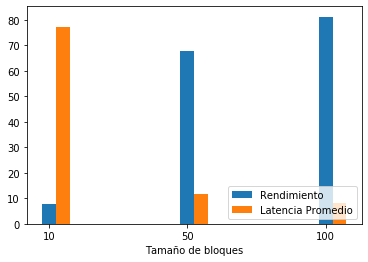
\includegraphics[scale=0.6]{Graphics/Resultado100TPS.png}
\caption{Evaluaci\'on de resultados para escenarios de 100 TPS.}
\label{Resultado100TPS}
\end{figure}


\clearpage

\section{An\'alisis de correlaci\'on entre los par\'ametros y los valores de latencia}

Para los escenarios con un flujo de transacciones de 10 y 100 TPS se discute el comportamiento de los par\'ametros: \emph{n\'umero de nodos pares} y \emph{tama\~no de bloque}, con relaci\'on a sus valores de latencia(m\'inima, m\'axima y promedio) en la red de Hyperledger Fabric.\\

Se comienza con la observaci\'on de los diagramas de dispersi\'on para asumir los criterios de correlaci\'on, que luego a partir del \emph{coeficiente de Spearman}[\cite{barrera2014uso}] son comprobados.\\

Las muestras de \emph{tama\~no de bloque} y \emph{n\'umero de nodos pares} son medidas en una escala ordinal. Por tanto, es posible usar el \emph{coeficiente de Spearman} para analizar su respectiva correlaci\'on con los valores de latencia.\\

Las hip\'otesis asumidas para el \emph{coeficiente de correlaci\'on de Spearman} son:
\begin{itemize}
\item $H_0$: Las muestras \emph{X} e \emph{Y} son mutuamente independientes.
\item $H_1$: Las muestras \emph{X} e \emph{Y} no son mutuamente independientes.
\end{itemize}

Para determinar los valores de $\rho$ y \emph{p-value} de \emph{Spearman} se utiliza el \emph{software} \emph{R} en su versi\'on 3.5.2.\\

Nivel de significancia: $\alpha = 0.05$.\\

Como criterio de decisi\'on se toma el rechazo de la hip\'otesis $H_0$ a partir del \emph{p-value}, si $\emph{p-value}\leq\alpha = 0.05$.\\

Para la interpretaci\'on de los valores se tuvo en cuenta la tabla \ref{tab:GradoCoeficiente} basada en \emph{Hern\'andez Sampieri y Fern\'andez Collado}, 1998.\\


En las figuras \ref{Rplot10TPS} y \ref{Rplot100TPS} por cada par \texttt{<x,y>} del conjunto formado por los par\'ametros y m\'etricas de latencia se dispone de un diagrama de dispersi\'on.\\
 

\newpage
\subsection{Escenario de 10 TPS}

Se observa en la figura \ref{Rplot10TPS} una leve relaci\'on de linealidad entre el n\'umero de nodos pares y cada m\'etrica de latencia. En el caso del tama\~no de los bloques resulta m\'as perceptible una relaci\'on de linealidad con respecto a la latencia promedio, en comparaci\'on al resto de las m\'etricas de latencia.\\

\begin{figure}[h]
\centering
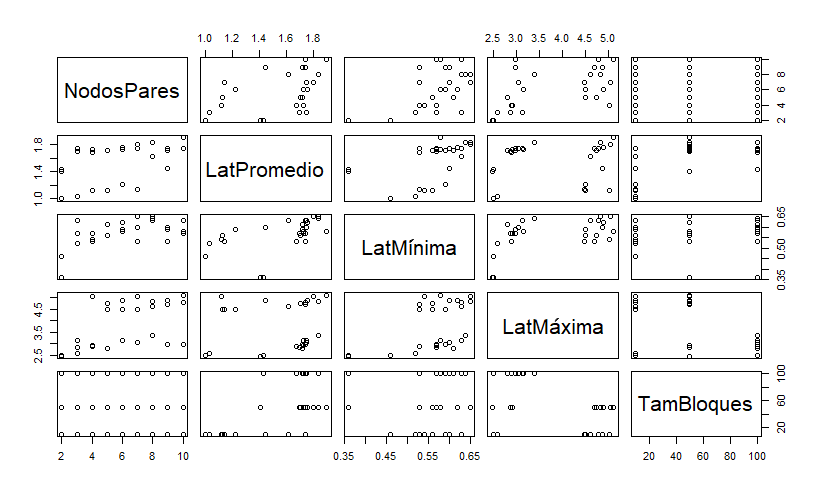
\includegraphics[scale=0.6]{Graphics/Rplot10TPS.png}
\caption{Diagrama de dispersi\'on para escenarios de 10 TPS.}
\label{Rplot10TPS}
\end{figure}

 
\subsubsection{An\'alisis de correlaci\'on entre el n\'umero de nodos pares y los valores de latencia}
Se realizaron las pruebas de correlaci\'on del \emph{coeficiente de Spearman} para evaluar la relaci\'on del n\'umero de nodos pares en la red de Fabric con relaci\'on a las m\'etricas de latencia. Los resultados se pueden ver en la tabla \ref{tab:CorrelacionNodosPares10TPS}.\\

\begin{table}[htb]
\centering
\rowcolors{2}{gray!20}{}
\scalebox{1}{\begin{tabular}{ c  c  c }
\hline
Latencia & $\rho$ & \emph{p-value} \\ 
\hline
\hline
M\'inima & 0.5337 & 0.0041 \\
M\'axima & 0.6144 & 0.0007 \\
Promedio & 0.5476 & 0.0031 \\
\hline
\end{tabular}}
\caption{Resultados de aplicar el \emph{coeficiente de correlaci\'on de Spearman} entre el n\'umero de nodos pares y las muestras de latencia en redes con un flujo de 10 TPS.}
\label{tab:CorrelacionNodosPares10TPS}
\end{table}

\newpage

Para las tres muestras de latencia sus valores de significancia (\emph{p-value}) son inferiores a 0.05, por tanto, se rechaza la hip\'otesis $H_0$ de independencia entre el n\'umero de nodos pares y las m\'etricas de latencia, pero como sus valores de $\rho$ est\'an en el rango de 0.51 a 0.75 su relaci\'on es de sentido positivo y magnitud considerable. Entonces con nivel de significaci\'on 0.05 las muestras de latencias dan evidencia de una relaci\'on lineal considerable con el n\'umero de nodos pares de la red.\\
  
De acuerdo al reciente an\'alisis podemos concluir que un aumento en el n\'umero de nodos pares puede ocasionar un aumento en los valores de latencia de la red de Fabric con bajos vol\'umenes de transacciones.\\


\subsubsection{An\'alisis de correlaci\'on entre el tama\~no de bloque y los valores de latencia}
Para el tama\~no de los bloques y los valores de latencia, se comprob\'o de igual forma, con el \emph{coeficiente de correlaci\'on de Spearman}, la existencia o no de una asociaci\'on lineal. En la tabla \ref{tab:CorrelacionTamBloques10TPS} se agrupan los resultados de las pruebas.\\

\begin{table}[h]
\centering
\rowcolors{2}{gray!20}{}
\scalebox{1}{\begin{tabular}{ c  c  c }
\hline
Latencia & $\rho$ & \emph{p-value} \\ 
\hline
\hline
M\'inima & 0.1489 & 0.4585 \\
M\'axima & -0.3379 & 0.0848 \\
Promedio & 0.5423 &  0.0035 \\
\hline
\end{tabular}}
\caption{Resultados de aplicar el \emph{coeficiente de correlaci\'on de Spearman} entre el tama\~no de los bloques y las muestras de latencia en redes con un flujo de 10 TPS.}
\label{tab:CorrelacionTamBloques10TPS}
\end{table}

Para las muestras de latencia m\'inima y latencia m\'axima se tiene un \emph{p-value} superior a 0.05, entonces se decide no rechazar la hip\'otesis de independencia entre el tama\~no de bloque y cada una de ellas, por lo que se asume la no existencia de una relaci\'on lineal de dichas m\'etricas con respecto al tama\~no de los bloques.\\

Con relaci\'on a la muestra de latencia promedio su \emph{p-value} es inferior a 0.05, por tanto, se rechaza la hip\'otesis $H_0$ de independencia entre el tama\~no de bloque y la latencia promedio. Entonces con nivel de significaci\'on 0.05 se asume una relaci\'on lineal entre las muestras. Como el valor de $\rho$ = 0.5423, presenta una relaci\'on lineal de sentido positivo y magnitud considerable para un valor de significaci\'on 0.05.\\ 

En resumen, de acuerdo a la muestra estudiada, un aumento del tama\~no de los bloques puede desencadenar un aumento en la latencia promedio de la red de Fabric, mientras sus valores sean mayores que el n\'umero de transacciones por segundo.\\



\newpage
\subsection{Escenario de 100 TPS}
Se puede observar en la figura \ref{Rplot100TPS} que el n\'umero de nodos pares con relaci\'on a los valores de latencia suponen una correlaci\'on, siendo m\'as perceptible con respecto a la latencia m\'inima. El tama\~no de los bloques, con relaci\'on a la latencia promedio y latencia m\'axima da muestra de una relaci\'on lineal negativa.\\

\begin{figure}[h]
\centering
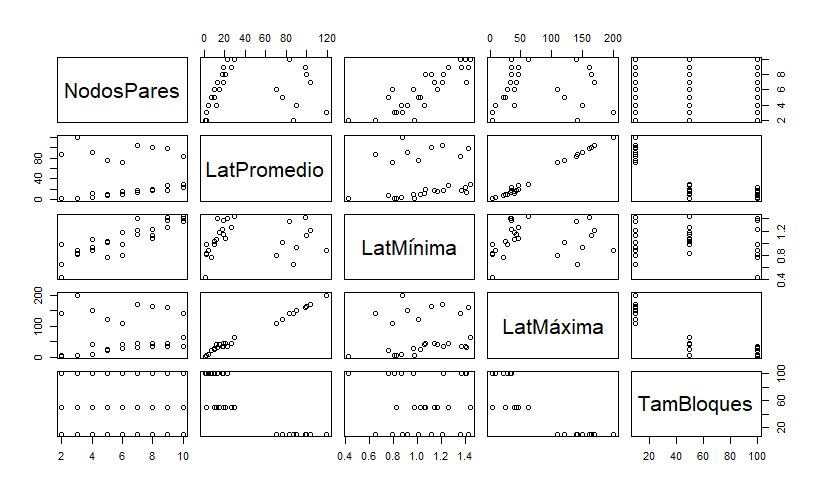
\includegraphics[scale=0.6]{Graphics/Rplot100TPS.png}
\caption{Diagrama de dispersi\'on para escenarios de 100 TPS.}
\label{Rplot100TPS}
\end{figure}

Como en el an\'alisis anterior, se verifican las observaciones de la figura \ref{Rplot100TPS} empleando el \emph{coeficiente de Spearman} de acuerdo a los mismos criterios.\\

\subsubsection{An\'alisis de correlaci\'on entre el n\'umero de nodos pares y los valores de latencia}
 En la tabla \ref{tab:CorrelacionNodosPares100TPS} se recogen los datos ofrecidos por las pruebas de correlaci\'on entre el n\'umero de nodos pares y las m\'etricas de latencia.\\
 
\begin{table}[h]
\centering
\rowcolors{2}{gray!20}{}
\scalebox{1}{\begin{tabular}{ c  c  c }
\hline
Latencia & $\rho$ & \emph{p-value} \\ 
\hline
\hline
M\'inima & 0.8545 & 1.409e-08 \\
M\'axima & 0.3462 & 0.07687 \\
Promedio & 0.4181 &  0.03001 \\
\hline
\end{tabular}}
\caption{Resultados de aplicar el \emph{coeficiente de correlaci\'on de Spearman} entre el n\'umero de nodos pares y las muestras de latencia en redes con un flujo de 100 TPS.}
\label{tab:CorrelacionNodosPares100TPS} 
\end{table} 

\newpage

Con respecto a los valores de latencia m\'inima se tiene un \emph{p-value} = 1.409e-08 $\ll$ 0.05, por tanto, se rechaza la hip\'otesis $H_0$ de independencia entre el n\'umero de nodos pares y la latencia m\'inima. Como su valor de $\rho$ = 0.8545 entonces con nivel de significaci\'on 0.05 se decide que existe una relaci\'on lineal de sentido positivo y magnitud fuerte entre las muestras.\\
 
En el caso de la latencia m\'axima se tiene un \emph{p-value} = 0.07687 $>$ 0.05 entonces no hay evidencia para rechaza la hip\'otesis $H_0$ de independencia entre el n\'umero de nodos pares y la latencia m\'axima. Por tanto, se decide no asumir una relaci\'on de linealidad entre las muestras.\\

Para la latencia promedio se tiene un \emph{p-value} = 0.03001 $<$ 0.05 entonces se rechaza la hip\'otesis $H_0$ de independencia entre el n\'umero de nodos pares y la latencia promedio. Como su valor de $\rho$ = 0.4181 est\'a en el rango de 0.51 a 0.75 se decide que entre las muestras existe una relaci\'on lineal de sentido positivo y magnitud considerable para un valor de significaci\'on 0.05.\\
 
 
Se concluye que un aumento del n\'umero de nodos pares en la red de Fabric aumenta la latencia promedio y latencia m\'inima para altos vol\'umenes de transacciones por segundo.\\

\subsubsection{An\'alisis de correlaci\'on entre el tama\~no de bloque y los valores de latencia}
En la tabla \ref{tab:CorrelacionTamBloques100TPS} se recogen los resultados de las pruebas de correlaci\'on del \emph{coeficiente de Spearman} entre una muestra de tama\~no de bloque y las muestras de latencia.\\

\begin{table}[h]
\centering
\rowcolors{2}{gray!20}{}
\scalebox{1}{\begin{tabular}{ c  c  c }
\hline
Latencia & $\rho$ & \emph{p-value} \\ 
\hline
\hline
M\'inima & 0 & 1 \\
M\'axima & -0.8212 & 1.538e-07 \\
Promedio & -0.7746 &  2.117e-06 \\
\hline
\end{tabular}}
\caption{Resultados de aplicar el \emph{coeficiente de correlaci\'on de Spearman} entre el tama\~no de los bloques y las muestras de latencia en redes con un flujo de 100 TPS.}
\label{tab:CorrelacionTamBloques100TPS}
\end{table}

\newpage

Los \emph{p-value} para la latencia m\'axima y latencia promedio son muy inferiores a 0.05, por tanto, se rechaza la hip\'otesis $H_0$ de independencia entre el tama\~no de los bloques con relaci\'on a la latencia m\'axima y m\'inima, a su vez sus valores de $\rho$ oscilan entre -0,76 y -0,90. Entonces se decide que existe una relaci\'on lineal de sentido negativo y magnitud fuerte entre el tama\~no de los bloques y las latencia m\'axima y promedio para un valor de significaci\'on 0.05.\\

Para la muestra de latencia m\'inima con un \emph{p-value} = 1 $\gg$ 0.05 se confirma que no existe evidencia para rechazar la hip\'otesis $H_0$ de independencia entre el tama\~no de los bloques y la latencia m\'inima. Por tanto, se decide que no hay una relaci\'on lineal entre las muestras.\\

Con este an\'alisis podemos concluir que, cuando el n\'umero de transacciones por segundo es superior a los valores de una muestra de tama\~no de bloque, un aumento del tama\~no de los bloques ocasiona una disminuci\'on en los valores de latencia m\'axima y latencia promedio de la red.\\


